% !TEX TS-program = pdflatex
% !TEX encoding = UTF-8 Unicode

% This is a simple template for a LaTeX document using the "article" class.
% See "book", "report", "letter" for other types of document.

\documentclass[12pt]{article} % use larger type; default would be 10pt

\usepackage[utf8]{inputenc} % set input encoding (not needed with XeLaTeX)

%%% Examples of Article customizations
% These packages are optional, depending whether you want the features they provide.
% See the LaTeX Companion or other references for full information.

%%% PAGE DIMENSIONS
\usepackage{geometry} % to change the page dimensions
\geometry{a4paper} % or letterpaper (US) or a5paper or....
% \geometry{margin=2in} % for example, change the margins to 2 inches all round
% \geometry{landscape} % set up the page for landscape
%   read geometry.pdf for detailed page layout information
\setlength{\parindent}{0pt}


% \usepackage[parfill]{parskip} % Activate to begin paragraphs with an empty line rather than an indent

%%% PACKAGES
\usepackage{booktabs} % for much better looking tables
\usepackage{array} % for better arrays (eg matrices) in maths
\usepackage{paralist} % very flexible & customisable lists (eg. enumerate/itemize, etc.)
\usepackage{verbatim} % adds environment for commenting out blocks of text & for better verbatim
%\usepackage{subfig} % make it possible to include more than one captioned figure/table in a single float
\usepackage{amsmath} %amsmath is part of AMS-LATEX bundles
\usepackage{amssymb}%symble
\usepackage{amsfonts}%font
\usepackage{amsthm}%provide theorem package
\usepackage{graphicx}
\usepackage{listings}
\lstset{breaklines} 
% These packages are all incorporated in the memoir class to one degree or another...
\usepackage[retainorgcmds]{IEEEtrantools} %In order to use IEEEeqnarray Environment
\usepackage{graphicx} % support the \includegraphics command and options
%\usepackage{indentfirst}%

%%% HEADERS & FOOTERS
\usepackage{fancyhdr} % This should be set AFTER setting up the page geometry
\pagestyle{fancy} % options: empty , plain , fancy
\renewcommand{\headrulewidth}{0pt} % customise the layout...
\lhead{}\chead{}\rhead{}
\lfoot{}\cfoot{\thepage}\rfoot{}

%%% SECTION TITLE APPEARANCE
\usepackage{sectsty}
\allsectionsfont{\sffamily\mdseries\upshape} % (See the fntguide.pdf for font help)
% (This matches ConTeXt defaults)

%%% ToC (table of contents) APPEARANCE
\usepackage[nottoc,notlof,notlot]{tocbibind} % Put the bibliography in the ToC
\usepackage[titles,subfigure]{tocloft} % Alter the style of the Table of Contents
\renewcommand{\cftsecfont}{\rmfamily\mdseries\upshape}
\renewcommand{\cftsecpagefont}{\rmfamily\mdseries\upshape} % No bold!
\usepackage{graphicx} % support the \includegraphics command and options
\usepackage{subfigure}%put multiple figure together, must use with package {tocloft}
%\usepackage{subcaption}
%\usepackage{subcaption}


%%%DEFINE UPRIGHT FONT MISSING FUNCTIONS????????????????????
\DeclareMathOperator{\argh}{argh}
\DeclareMathOperator*{\nut}{Nut}

%%%DEFINE NEW COMMANDS
\newcommand{\ud}{\,\mathrm{d}}

%%%DEFINE THEOREM
%\theoremstyle{definition} 
\theoremstyle{definition}\newtheorem{law}{Law}
\theoremstyle{plain}\newtheorem{jury}[law]{Jury}
\theoremstyle{remark}\newtheorem{juu}{Juu}
\theoremstyle{definition}\newtheorem{kuu}[law]{Kuu}
\theoremstyle{definition}\newtheorem{muu}{Muu}[section]
\theoremstyle{definition}\newtheorem{honoluu}{Honoluu}[section]
\theoremstyle{definition}\newtheorem{konoluu}[muu]{Konoluu}

%%% END Article customizations

%%% The "real" document content comes below...

\title{\textbf{ \begin{LARGE}Neural Network\end{LARGE}}\\ [0ex]\begin{Large} Homework 2 \end{Large} }
\author{Ning Ma, A50055399}
\date{} % Activate to display a given date or no date (if empty),
         % otherwise the current date is printed 

\begin{document}
\maketitle
\section{Linear Rgression}

{\bf 1.}
Since $\epsilon \sim  \mathcal{N}(\mu = 0,\sigma^2)$, we have $\mathrm{P}(t|x;\theta) = \mathcal{N}(f(x,\theta), \sigma^2)$. Thus, for iid samples, we have
\begin{IEEEeqnarray}{rCl}
\mathrm{P}(T|X;\theta) & = & \prod_{i = 1}^{N}\frac{1}{\sqrt{2\pi\sigma^2}}\mathrm{exp}\left (-\frac{(t^{(i)} - f(x^{(i)},\theta))^2}{2\sigma^2}\right )
\end{IEEEeqnarray}
The optimal parameter $\theta$ should maximize the above posterior. Since $\mathbf{log}$ is a monotonically increasing function, it is equivalent to maximize  $\mathrm{log} \ \mathrm{P}(T|X;\theta)$
\begin{IEEEeqnarray}{rCl}
\mathrm{log} \ \mathrm{P}(T|X;\theta) & \sim & -\sum_{i = 1}^N(t^{(i)} - f(x^{(i)}, \theta))^2
\end{IEEEeqnarray}
which is equivalent to minimize $\sum_{i = 1}^N(t^{(i)} - f(x^{(i)}, \theta))^2$ which is the $\mathrm{SEE}$.

In conclusion, in this special problem, minimize the $\mathrm{SSE}$ is equivalent to maximize the posterior of observation.




\section{Multilayer Perceptron}
{\bf (a)}
The cross entropy loss function for softmax regression is 
\begin{equation}
E = -\sum_{l = 0}^{K - 1}1_{\{label = l\}}\mathrm{log} \ y_l
\end{equation}
where $y_l = \frac{\mathrm{exp}(a_l)}{\sum_{m = 0}^{K - 1}\mathrm{exp}(a_m)}$


For the output layer, we have 
\begin{IEEEeqnarray}{rCl}
\delta_k & = & -\frac{\partial E}{\partial a_k} = -\sum_l \frac{\partial E}{\partial y_l}\frac{\partial y_l}{\partial a_k}\\
& = & -\sum_l-\frac{1_{\{label= l\}}}{y_l}(y_l\delta_{lk} - y_ly_k)\\
& = & \sum_l 1_{\{label = l\}}(\delta_{lk} - y_k)\\
& = & \sum_{l}\delta_{lk}1_{\{label = l\}} - y_k\sum_{l}1_{\{label = l\}}\\
& = & 1_{\{label = k\}} - y_k = t_k - y_k
\end{IEEEeqnarray}

For the hidden layer, $y_j = g(a_j)$, we have 
\begin{IEEEeqnarray}{rCl}
\delta_j & = & -\frac{\partial E}{\partial a_j} = -\sum_k \frac{\partial E}{\partial a_k}\frac{\partial a_k}{\partial a_j}\\
& = & \sum_k\delta_k\frac{\partial a_k}{\partial a_j} = \sum_k\delta_k\frac{\partial a_k}{\partial y_j}\frac{\partial{y_j}}{\partial{a_j}}\\
& = & \sum_k\delta_k\frac{\partial \sum_l w_{lk}y_l}{\partial y_j}y_j^{'} = \sum_k\delta_kw_{jk}y_j^{'}\\
& = & y_j^{'}\sum_k\delta_kw_{jk}
\end{IEEEeqnarray}
where $\delta_k$ has been computed from the output layer.

{\bf (b)}
For the output layer, we have 
\begin{IEEEeqnarray}{rCl}
w_{jk} & = & w_{jk} - \alpha\frac{\partial E}{\partial w_{jk}} = w_{jk} - \alpha\frac{\partial E}{\partial a_k}\frac{\partial a_k}{\partial w_{jk}}\\
& = & w_{jk}  + \alpha \delta_k \frac{\partial \sum_l w_{lk}y_l}{\partial w_{jk}}\\
& = & w_{jk} + \alpha \delta_k y_j
\end{IEEEeqnarray}

For the hidden layer, we have
\begin{IEEEeqnarray}{rCl}
w_{ij} & = & w_{ij} - \alpha\frac{\partial E}{\partial w_{ij}} = w_{ij} - \alpha\frac{\partial E}{\partial a_j}\frac{\partial a_j}{\partial w_{ij}}\\
& = & w_{ij}  + \alpha \delta_j \frac{\partial \sum_l w_{lj}x_l}{\partial w_{ij}}\\
& = & w_{ij} + \alpha \delta_j x_i
\end{IEEEeqnarray}
where we have already computed the $\delta_k$ and $\delta_j$ in part (a).

{\bf (c)}
For the output layer, since $ w_{jk} = w_{jk} + \alpha\delta_k y_j$, we have
\begin{IEEEeqnarray}{rCl}
W_{HO} = W_{HO} + \alpha y^{(j)} \otimes \delta^{(k)}
\end{IEEEeqnarray}
where $y^{(j)}$ is a column-vector output from hidden layer, $\delta^{(k)}$ is a column-vector $\delta$ from the output layer, and $\otimes$ is an outer product operator.\\

Similarly, for the hidden layer, since $w_{ij} =  w_{ij} + \alpha \delta_j x_i$, we have
\begin{IEEEeqnarray}{rCl}
W_{IH} = W_{IH} + \alpha x^{(i)} \otimes \delta^{(j)}
\end{IEEEeqnarray}
where $x^{(i)}$ is a column-vector input, $\delta^{(j)}$ is a column-vector $\delta$ from the  hidden layer, and $\otimes$ is an outer product operator.\\

Since $\delta_j = y_j^{'}\sum_k\delta_kw_{jk}$, we have 
\begin{IEEEeqnarray}{rCl}
\delta^{(j)} = (y^{'})^{(j)}\odot(W_{HO}\bullet\delta^{(k)})
\end{IEEEeqnarray}
where $\odot$ is an element-wise multiplication operator.
Thus, we have 
\begin{IEEEeqnarray}{rCl}
W_{IH} = W_{IH} + \alpha x^{(i)} \otimes \left ( (y^{'})^{(j)}\odot(W_{HO}\bullet\delta^{(k)}) \right )
\end{IEEEeqnarray}

{\bf (d)}
\begin{enumerate}
\item[i.]
See code 'DataProcess.py' for detail
\item[ii.]
I choose a few parameters and the difference is smaller than $10^{-5}$. Since I also get fine results in the following questions, I think my gradient is correct.
\item[iii.]
We can see from Figure \ref{fig:notrick} that the training and test accuracy increases rapidly with number of iteration.
\begin{figure}[h!]
\centering
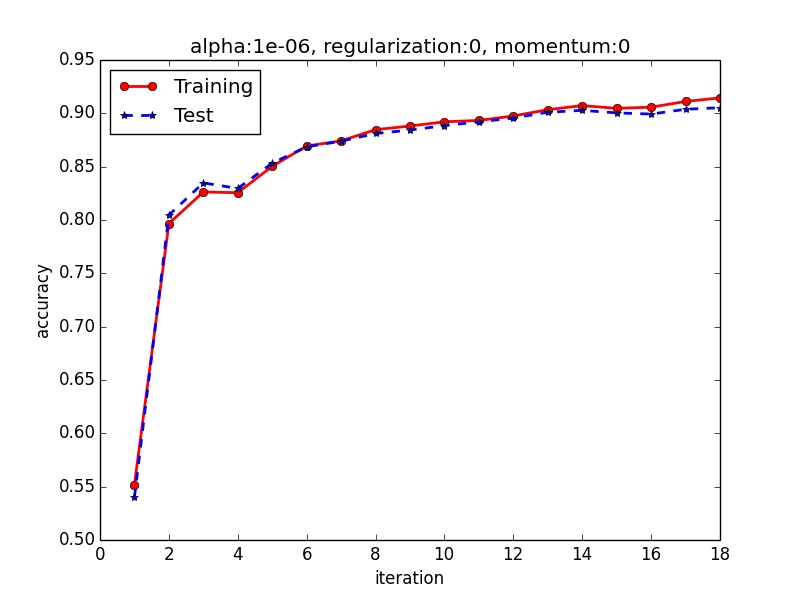
\includegraphics[width=1\textwidth]{sigmoid.png}
\caption{(d).iii. Sigmoid without trick}
\label{fig:notrick}
\end{figure} 
\end{enumerate}

{\bf (e)}
From Figure~\ref{fig:reg}, we can see that with regularization, the accuracy also increases rapidly with number of iterations. Large regularization can prevent from overfitting but make the model less powerful. With regularization, the gradient converges faster than the one without any trick. However, as regularization parameter increases, the accuracy decreases a little bit because the model is less powerful.
 \begin{figure}[h!]
\centering
\subfigure[regularization: 0.001]{%
  \includegraphics[width=0.8\textwidth]{regularization1.png}
  \label{fig:reg1}}
\quad
\subfigure[regularization: 0.0001]{%
  \includegraphics[width=0.8\textwidth]{regularization2.png}
  \label{fig:reg2}}
\caption{(e). Different regularization}
\label{fig:reg}
\end{figure}

{\bf (f)}
From Figure~\ref{fig:momentum}, the accuracy also increases with number of iterations but increases slower than previous cases. This is because momentum intends to dump big jumps during gradient descent process.
\begin{figure}[h!]
\centering
\includegraphics[width=1\textwidth]{momentum.png}
\caption{(f). With momentum}
\label{fig:momentum}
\end{figure} 


{\bf (g)}
Figure~\ref{fig:fun} shows how accuracy changes with number of iteration for different functions. We can see that $sigmoid$ activation function converges more quickly than $tanh$ and $ReLu$, and $tanh$ converges quicker than $ReLu$. This is because $ReLu$ is a linear increasing function, while $sigmod$ and $tanh$ are nonlinear functions and become saturated when input is large 
\begin{figure}[h!]
\centering
\subfigure[sigmoid]{%
  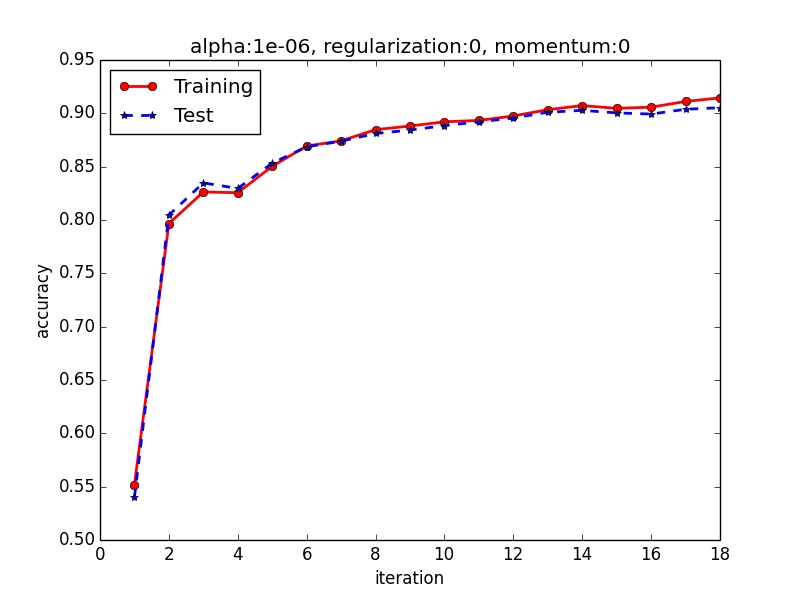
\includegraphics[width=0.5\textwidth]{sigmoid.png}
  \label{fig:sigmoid}}
\quad
\subfigure[tanh]{%
  \includegraphics[width=0.5\textwidth]{tanh.png}
  \label{fig:tanh}}
\quad
\subfigure[ReLu]{%
  \includegraphics[width=0.5\textwidth]{ReLu.png}
  \label{fig:relu}}
\caption{(g). Different activation functions}
\label{fig:fun}
\end{figure}

{\bf (h)}
\begin{enumerate}
\item[i.]
From Figure~\ref{fig:numhidden}, we can see that the accuracy increases with number of hidden units. It makes sense because the neural network becomes more powerful when the number of hidden units is larger. However, we can see that the accuracy improvement is very small. So, it is not always necessary to have a very large number of hidden units to increase slight accuracy but sacrifice a lot of computational time.

\begin{figure}[h!]
\centering
\subfigure[Half hidden units]{%
  \includegraphics[width=0.8\textwidth]{HalfHiddenUnits.png}
  \label{fig:half}}
\quad
\subfigure[Double hidden units]{%
  \includegraphics[width=0.8\textwidth]{DoubleHiddenUnits.png}
  \label{fig:double}}
\caption{(h).i. Different number of hidden units}
\label{fig:numhidden}
\end{figure}

\item[ii.]
From Figure~\ref{fig:twolayer}, we can see that, though the number of weights are similar, the accuracy increases with number of layers. Although, this double hidden layer network has similar number of weight, it has more complicated structure, and thus provides more powerful representation. So, when increasing hidden units does not increase the accuracy significantly, we can consider changing the structure of the network.
\begin{figure}[h!]
\centering
\includegraphics[width=1\textwidth]{twoHiddenLayer.png}
\caption{(h).ii. Two Hidden Layer }
\label{fig:twolayer}
\end{figure} 
\end{enumerate}


\newpage
\newpage

\section{Appendix}
The following is the  source code\\
\lstinputlisting[language=Python]{DataProcess.py}
\lstinputlisting[language=Python]{FunctionGradient.py}
\lstinputlisting[language=Python]{multilayerNN.py}
\lstinputlisting[language=Python]{twoHiddenLayerNN.py}
\end{document}
